\section{Physics goals}
We will measure the differential cross section for the charged current interaction on $\mathrm{H_2O}$ and Hydrocarbon(CH)).
The water-scintillator mass ratio of the Wagasci module is as high as 5:1 and the high purity measurement
of the cross section on $\mathrm{H_2O}$ is possible.
One experimental option is to remove water from one of the two Wagasci modules. 
The water-out WAGASCI module will allow to measure pure-CH target interactions with very low momentum-threshold for protons.
It will also benefit to subtract the background from interaction with scintillator in the water target measurement.
Another option is to add the T2K proton module which is fully made of plastic scintillators.
It will allow the high statistics comparison of cross section between $\mathrm{H_2O}$ and CH and also comparison
with the ND280 measurement. The actual configuration will be optimized with detailed MC simulation by 2018 Summer.

Our setup allows the measurements of inclusive and also exclusive channels such as
1-$\mu$, 1-$\mu 1p$, 1-$\mu 1\pi{\pm} np$ samples, former two of which are mainly caused by the quasi-elastic and
2p2h interaction and the latter is mainly caused by resonant or coherent pion production and deep elastic scattering.
In general, an accelerator produced neutrino beam spectrum is wide and the energy reconstruction
somehow rely on the neutrino interaction model.
Therefore, recent neutrino cross section measurement results including those from T2K are given
as a flux-integrated cross section rather than cross sections as a function of the neutrino energy to avoid the model dependency.
We can provide the flux-averaged cross section.
In addition, by combining our measurements with those at ND280, model-independent extraction of the cross section
for narrow energy region becomes possible.
This method was demonstrated in \cite{Abe:2015biq} and also proposed by P** (NUPRISM).

\subsection{Expected number of events}
Expected number of neutrino events after the event selections is evaluated with Monte Carlo simulations as we will discuss in Section \ref{sec:mc_study}.
In the neutrino-mode, $4.2 \times 10^{3}$, $1.1 \times 10^{3}$ and $3.8 \times 10^{3}$ CC neutrino events are expected in the water-in WAGASCI module, the water-out WAGASCI module and the INGRID proton module after the selections with $0.5\times 10^{21}$ POT, and its purities are 78.0 \%, 97.5 \% and $\sim 98 \%$.
In the antineutrino-mode, $1.7 \times 10^{3}$, $0.4 \times 10^{3}$ and $1.5 \times 10^{3}$ CC antineutrino events are expected in the water-in WAGASCI module, the water-out WAGASCI module and the INGRID proton module after the selections with $0.5\times 10^{21}$ POT, and its purities are 59.5 \%, 74.4 \% and $\sim 74 \%$.


Statical errors of flux integrated CC-inclusive neutrino cross section measurements on H$_{2}$O (full acceptance) and CH targets (forward acceptance)
will be 1.5 \% and 1.6 \% with $0.5\times 10^{21}$ POT in the neutrino-mode.
Statical errors of flux integrated CC-inclusive antineutrino cross section measurements on H$_{2}$O (full acceptance) and CH targets (forward acceptance)
will be 2.4 \% and 2.5 \% with $0.5\times 10^{21}$ POT in the antineutrino-mode.


Statical errors of flux integrated H$_{2}$O to CH CC-inclusive neutrino cross section ratio measurement 
will be 3.1 \% (full acceptance) and 2.3 \% (forward acceptance) with $0.5\times 10^{21}$ POT in the neutrino-mode.
Statical errors of flux integrated H$_{2}$O to CH CC-inclusive antineutrino cross section ratio measurement will be 5 \% (full acceptance) and 3.7 \% (forward acceptance) with $0.5\times 10^{21}$ POT in the antineutrino-mode.


\subsection{Pseudo-monochromatic beam by using different off-axis fluxes}
The off-axis method gives narrower neutrino spectrum, and the peak energy is lower for larger off-axis angle.
There still remains high energy tail mainly due to neutrinos from Kaon decay.
The off-axis angle of the Wagasci location is 1.5 degree and different from the ND280 2.5 degree.
Top two plots of Fig.~\ref{fig:fluxsubtfhc} show the energy spectra of fluxes and neutrino interaction events
at these two different location.
The high energy tail of ND280 flux can be somehow subtraction by using the Wagasci measurement.
The low energy part of the Wagasci flux can be also subtracted by using the ND280 measurement.
Bottom two plots of Fig.~\ref{fig:fluxsubtfhc} demonstrate this method.
We can effectively get two fluxes, from 0.2 GeV to 0.9 GeV and 0.6 GeV and 2 GeV
and measure flux-integrated cross section for these two fluxes.

\begin{figure}[tbh]
\begin{center}
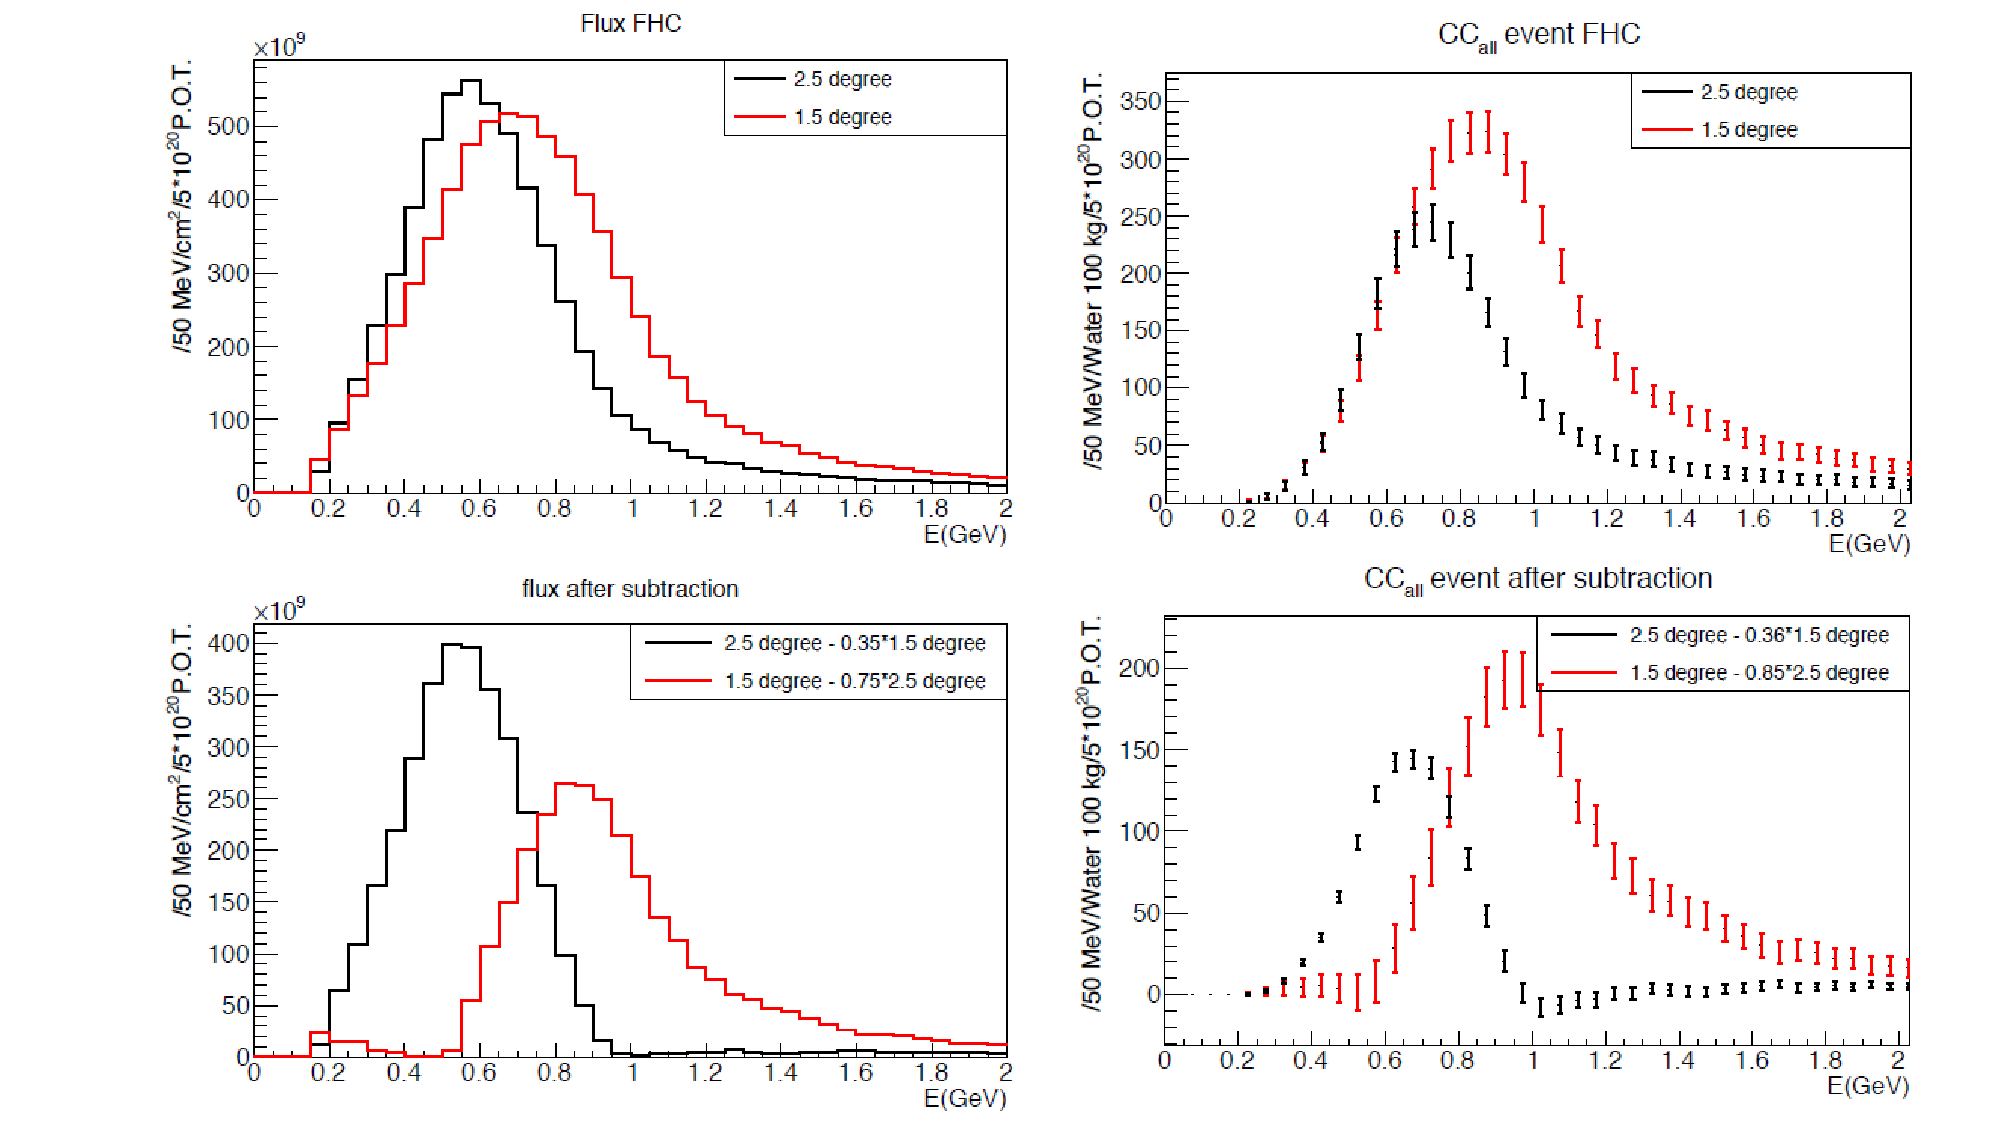
\includegraphics[width=\textwidth]{fig/fluxsubtractFHC.pdf}
\end{center}
\caption{Energy spectra obtained by using different off-axis angle fluxes.
  Top two plots show the fluxes(left) and spectra of interaction events (right) for ND280 (off-axis 2.5 degree) and Wagasci (off-axis 1.5 degree). Bottom two plots show the fluxes (left) and spectra of interaction events (right) obtained by
  subtraction of fluxes at ND280 and Wagasci.
  The error bar is for the statistical error and those in the bottom right plot is obtained assuming the statistical error
  for ND280 measurement is much smaller than that of Wagasci experiment.
}
\label{fig:fluxsubtfhc}
\end{figure}


Statical errors of flux integrated CC-inclusive neutrino cross section measurements on H$_{2}$O (forward acceptance) and CH targets (forward acceptance) with the pseudo-monochromatic beam
will be 2 \% and 1.9 \% with $0.5\times 10^{21}$ POT in the neutrino-mode.
Statical errors of flux integrated CC-inclusive antineutrino cross section measurements on H$_{2}$O (forward acceptance) and CH targets (forward acceptance) with the pseudo-monochromatic beam
will be 3 \% and 2.8 \% with $0.5\times 10^{21}$ POT in the neutrino-mode.


\subsection{Subjects Wagasci can contribute}
In T2K experiment, neutrinos interact with bound nucleons in relatively heavy nuclei (Carbon and Oxygen), so the cross-section is largely affected by nuclear effects.
The nuclear effects are categorized as nucleons' momentum distribution in nucleus, interactions with  correlated pairs of nucleons in nucleus (two particles-two holes, 2p2h), collective nuclear effects 
%calculated with Random Phase Approximation (RPA) 
and final state interactions (FSI) of secondary particles in the nuclei after the initial neutrino interactions.


The 2p2h interactions mainly happen through $\Delta$ resonance interactions following a pion-less decay and interactions with a correlated nucleon pair.
The 2p2h interactions are observed in electron scattering experiments \cite{escattering} where the 2p2h events observed in the gap between Quasi-Elastic region and Pion-production region as shown in Fig. \ref{fig:electrono_scattering_data}.
Neutrino experiments also attempt to measure the 2p2h interactions, but separation of the QE peak and the 2p2h peak is more difficult because transferred momentum (p) and energy (w) are largely affected by  neutrino energies which cannot be determined event-by-event in the wide energy spectrum of the accelerator neutrino beam.
Our model-independent narrow neutrino spectra extracted from combined analyses of our data and ND280 data are ideal for searching the 2p2h interaction because clearer separation of the QE peak and the 2p2h peak is expected.
Another way to observe the 2p2h interaction is direct measurement of proton tracks in CC0$\pi$ sample with low detection threshold and full acceptance.
Fig. \ref{fig:2p2h_proton_multiplicity} shows proton multiplicities after FSI in CCQE events and 2p2h events, and Fig. \ref{fig:2p2h_proton_angle} shows opening angles among two proton tracks in the same samples.
The water-out Wagasci can provide good sample for the 2p2h interaction search because its low density medium enables the detection of low momentum protons in addition to the full acceptance.

\begin{figure}[tbh]
\begin{center}
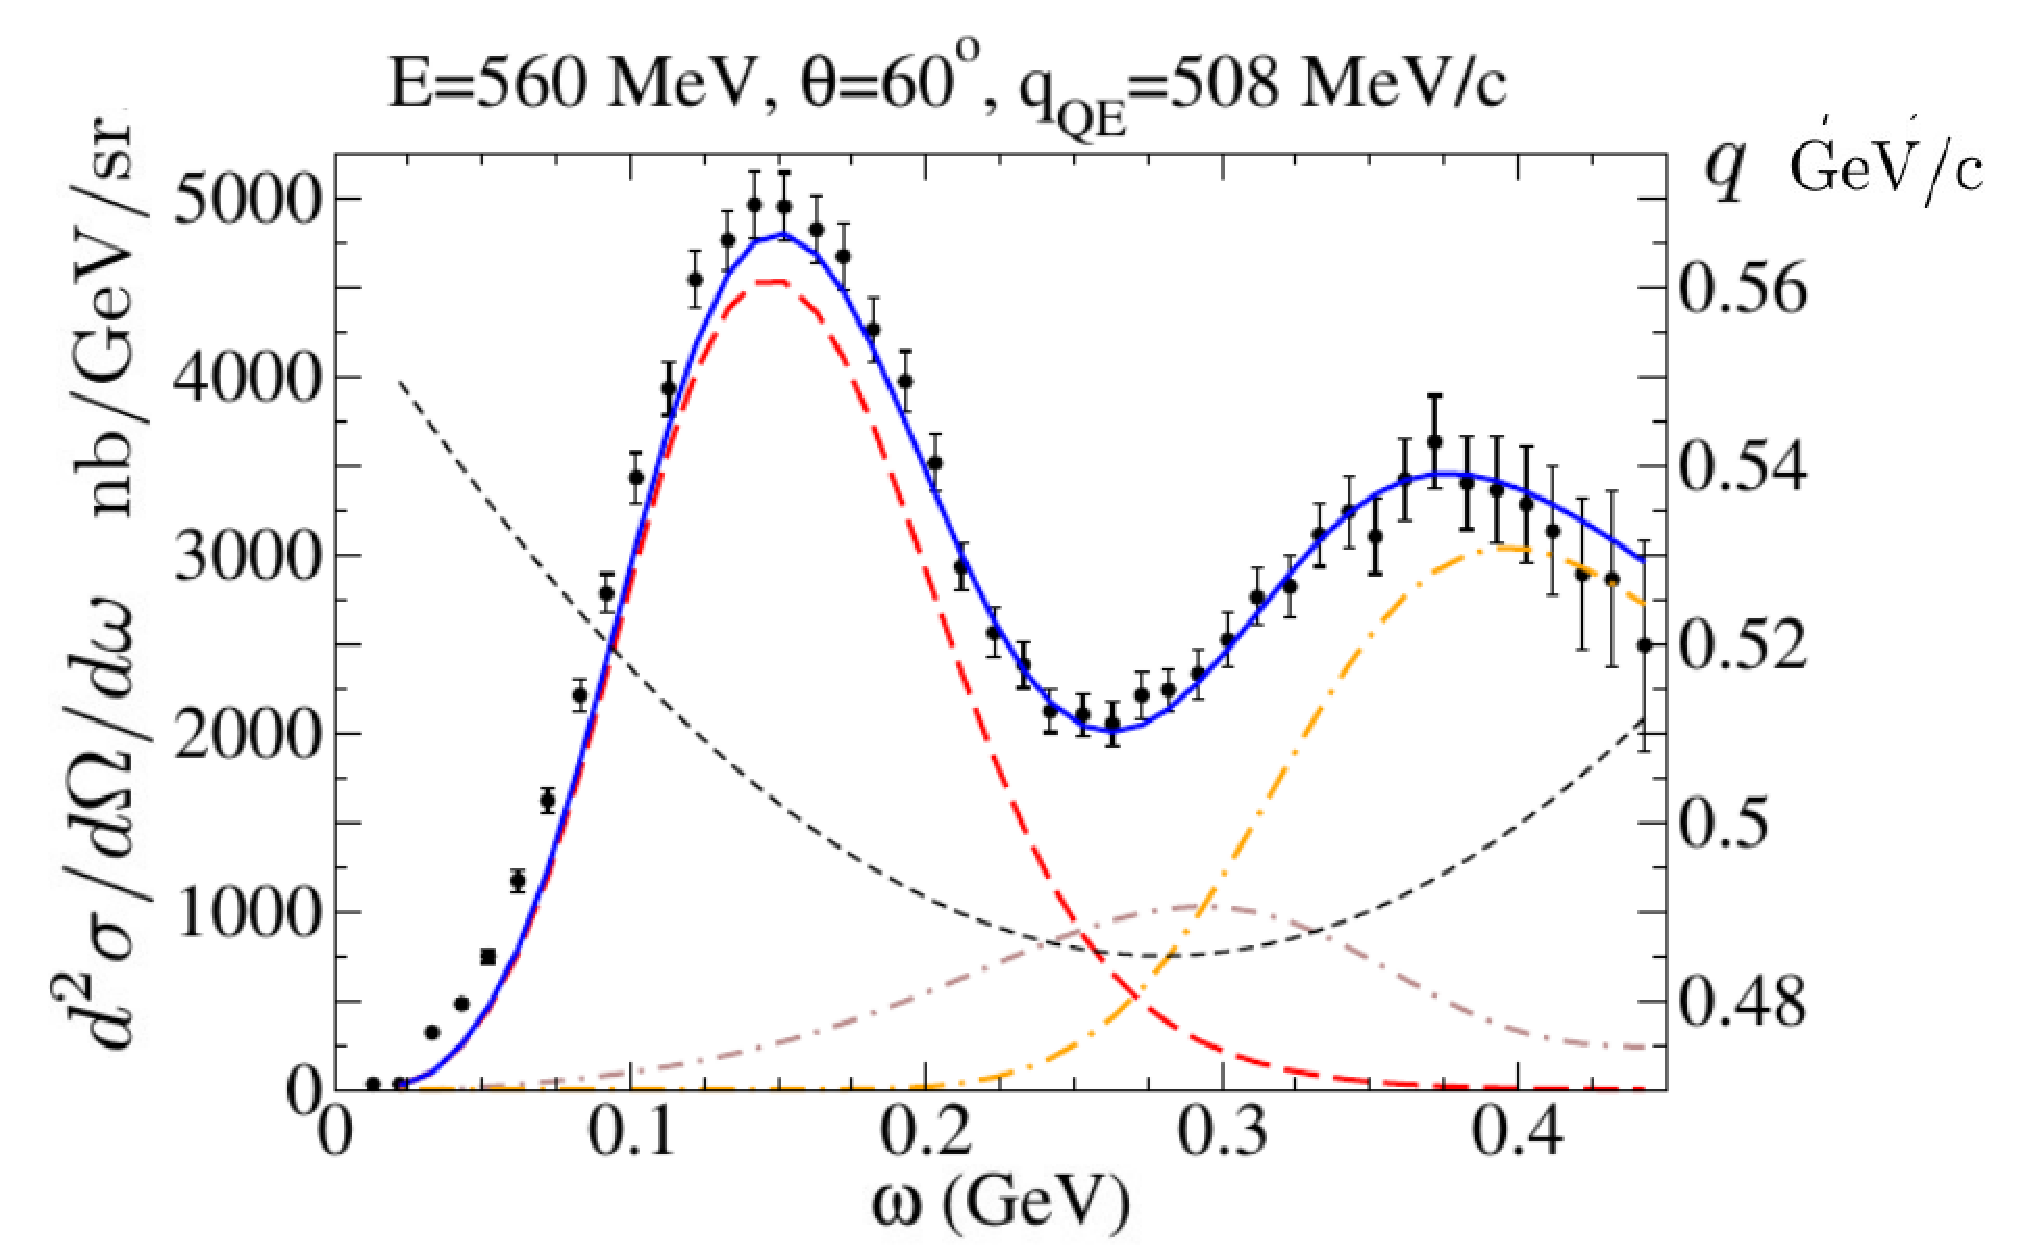
\includegraphics[width=0.8\linewidth]{fig/escattering.pdf}
\end{center}
\caption{
Comparison of inclusive $^{12}$C(e,e') cross sections and predictions of the QE-SuSAv2 model (long-dashed red line), 2p-2h MEC model (dot-dashed brown line) and inelastic-SuSAv2 model (long dot-dashed orange line) (from Ref. \cite{escattering}).
The sum of the three contributions is represented with a solid blue line.
The q dependence with w is also shown (short-dashed black line.)
}
\label{fig:electrono_scattering_data}
\end{figure}

\begin{figure}[tbh]
\begin{center}
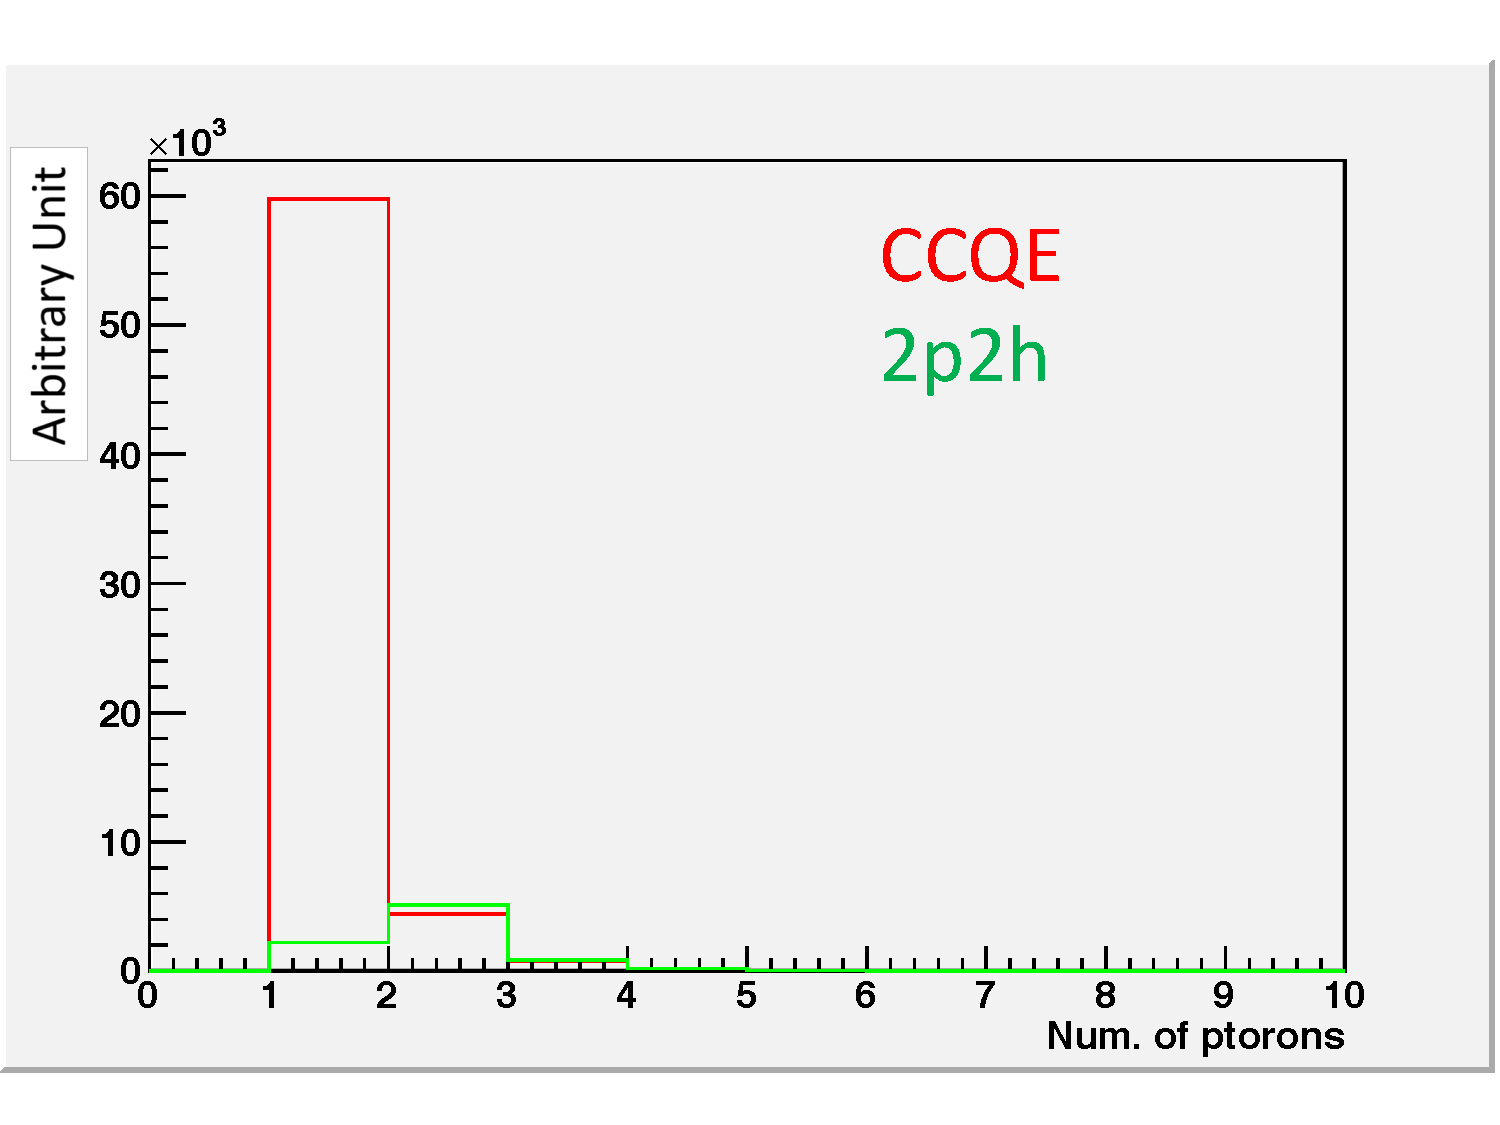
\includegraphics[width=0.6\linewidth]{fig/2p2h_proton_multiplicity.pdf}
\end{center}
\caption{
Proton multiplicities after FSI in CCQE events and 2p2h events.
}
\label{fig:2p2h_proton_multiplicity}
\end{figure}

\begin{figure}[tbh]
\begin{center}
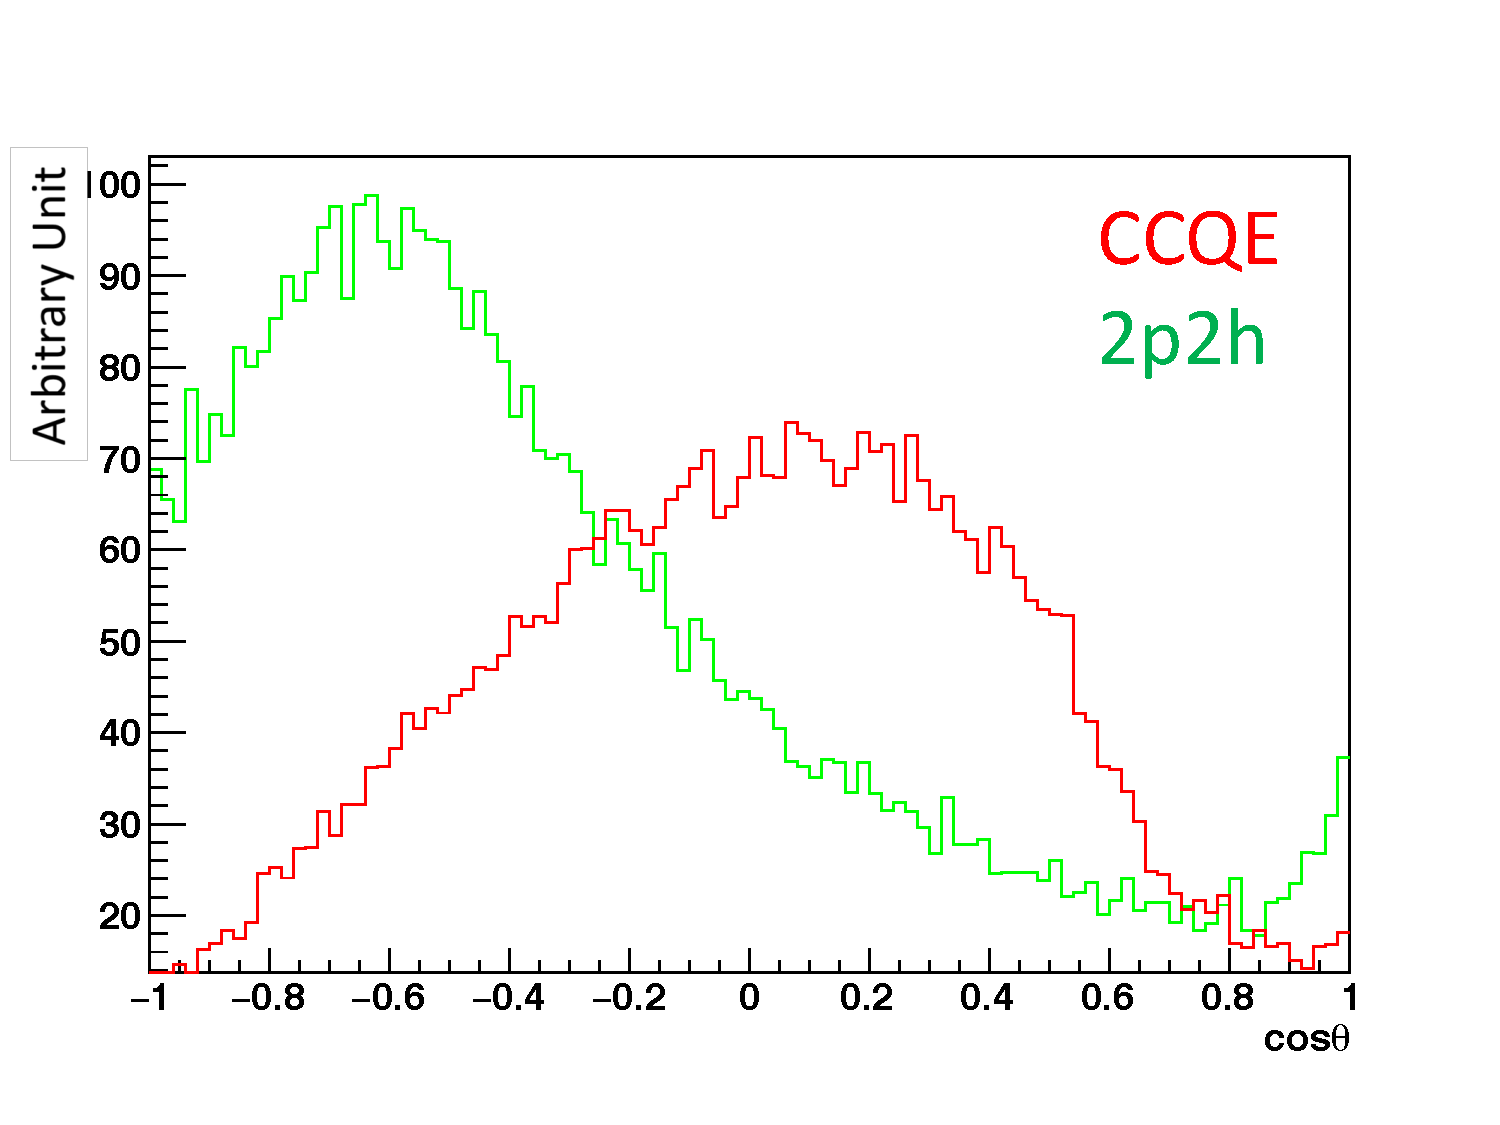
\includegraphics[width=0.6\linewidth]{fig/2p2h_proton_angle.pdf}
\end{center}
\caption{
Opening angles among two proton tracks after FSI in CCQE events and 2p2h events.
}
\label{fig:2p2h_proton_angle}
\end{figure}


% The corrections from collective nuclear effects calculated by RPA as a function of $Q^{2}$ are shown in Fig. \ref{fig:effect_rpa}.
% The $Q^{2}$ dependence of the correction can be tested by measuring angular distribution of muons in CC1-$\mu$ and CC1-$\mu 1p$ events.
% The uncertainties of the corrections in low (high) $Q^{2}$ regions can be constrained by observing the events with a forward-going (high-angle) muon, so it is essential to measure muon tracks with full acceptance.
There are various models which describe the collective nuclear effects \cite{collective_nuclear_effect}.
The $Q^{2}$ dependence of the effects can be tested by measuring angular distribution of muons in CC1-$\mu$ and CC1-$\mu 1p$ events.
The uncertainties of the effects in low (high) $Q^{2}$ regions can be constrained by observing the events with a forward-going (high-angle) muon, so it is essential to measure muon tracks with full acceptance.
% Based on the measurement, we can evaluate the models and determine model parameters.


T2K experiment is starting to use $\nu_{e}$ CC1$\pi$ events for its CP violation search to increase the statistics.
One of the biggest uncertainty of the CC1$\pi$ sample comes from the final state interactions of pions in the nuclei after the initial neutrino interactions because they change the multiplicity, charge and kinematics of the pions.
The multi-pion production events can be migrated into the CC1$\pi$ sample due to the FSIs, and they become important backgrounds.
We can constrain the uncertainties from the pion FSIs by measuring pion rescattering in the detector and pion multiplicity in $\nu_{\mu}$ CCn$\pi$ sample with low detection threshold and full acceptance for pion tracks.
The water-out WAGASCI can provide good sample for the pion FSI studies because its low density medium enables the detection of low momentum pions in addition to the full acceptance.

